% template from http://nook.cs.ucdavis.edu/~koehl/Teaching/ECS20/homeworks.html
\documentclass[11pt]{article}
\usepackage{amsthm,amsmath, amssymb}
\setlength{\oddsidemargin}{0in}
\setlength{\evensidemargin}{0in}
\setlength{\textheight}{9.0in}
\setlength{\textwidth}{6.5in}
\setlength{\topmargin}{-0.5in}
\usepackage{graphicx}
\usepackage{listings}
\lstset{xleftmargin=.25in}  % https://tex.stackexchange.com/questions/10828/
\usepackage{multicol}
\usepackage{courier}
\usepackage{verbatim}
\lstset{basicstyle=\footnotesize\ttfamily,breaklines=true}
\usepackage{fancyhdr}
\usepackage{indentfirst}
\pagestyle{fancy}
\usepackage{hyperref}
\usepackage{tikz}

% Due Jun 5
\newcommand{\titleVar}{ECS 175 Fall 2019 - Assignment 1 Manual}

\lhead{\titleVar{}} \chead{} \rhead{lxylxy123456}
\lfoot{} \cfoot{\thepage} \rfoot{}
\renewcommand{\headrulewidth}{0pt}
\renewcommand{\footrulewidth}{0pt}
\setlength\headsep{0.333in}
\title{\bf \titleVar{}}
\author{lxylxy123456 (https://github.com/lxylxy123456/)}

\newcommand{\insertGraph}[3]{

  \centerline{\includegraphics[scale=#1]{#2}}

  \centerline{#3}

}

\newcommand{\insertTwoGraphs}[3]{

  \begin{multicols}{2}

  \insertGraph{#1}{#2.png}{#2}

  \insertGraph{#1}{#3.png}{#3}

  \end{multicols}

}

\begin{document}
\maketitle

\renewcommand\thesubsection{\arabic{section}.\Alph{subsection}}

This work is licensed under a Creative Commons
Attribution-NonCommercial-NoDerivatives 4.0 International License.
(http://creativecommons.org/licenses/by-nc-nd/4.0/)

\section{Run}

Put data file at \lstinline{test_scene} in current working directory. 
 Then use \lstinline{./Project1} to run the project. 


\section{Menu}

\subsection{Introduction}

There is a right-click menu in the system, also all functions can be invoked
 using keyboard. For example, \lstinline{a} means just pressing key ``A'' and
 \lstinline{A} means press ``Shift + A''. The \lstinline{stdout} at the terminal
 will show important instructions and information. 

\subsection{Bresenham / DDA}

Right click menu's first option allows switching the line drawing algorithm
 between Bresenham and DDA. Also use keyboard \lstinline{b} or \lstinline{d}.

\subsection{Fill / Draw}

Right click menu's second option allows switching between filling (with interior
 of polygon) and drawing (only drawing edges). Also use keyboard \lstinline{f}.

\subsection{Clipping}

Right click menu's third option enables clipping. Please follow these steps. 
\begin{enumerate}
\item Click on menu's ``Clip'' or press keyboard \lstinline{c}. 
\item Go to a corner of the clipping window, press and hold the left mouse
	button. 
\item Drag the mouse to the other corner of the clipping window, then release
	left mouse button. 
\end{enumerate}

Right click menu's fourth option ``No Clip'' disables clipping. Also use
 keyboard \lstinline{C} (Shift + C).

See the figure below. 

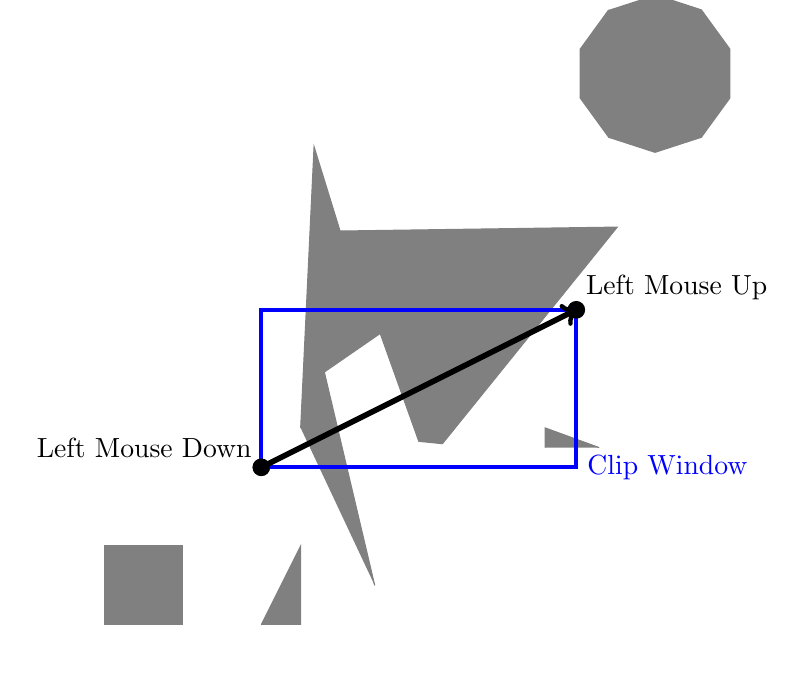
\begin{tikzpicture}

\def\s{0.1}

\filldraw [color=gray]
(25.000000 * \s, 25.000000 * \s) --
(26.700000 * \s, 60.700000 * \s) --
(30.000000 * \s, 50.000000 * \s) --
(65.200000 * \s, 50.500000 * \s) --
(43.000000 * \s, 23.000000 * \s) --
(40.000000 * \s, 23.300000 * \s) --
(35.100000 * \s, 37.000000 * \s) --
(28.000000 * \s, 32.100000 * \s) --
(34.400000 * \s,  5.000000 * \s);

\filldraw [color=gray]
( 0.000000 * \s,  0.000000 * \s) --
(10.000000 * \s,  0.000000 * \s) --
(10.000000 * \s, 10.000000 * \s) --
( 0.000000 * \s, 10.000000 * \s);

\filldraw [color=gray]
(56.048951 * \s, 22.500006 * \s) --
(56.048951 * \s, 24.999988 * \s) --
(62.902098 * \s, 22.500006 * \s);

\filldraw [color=gray]
(25.000000 * \s,  0.000000 * \s) --
(25.000000 * \s, 10.000000 * \s) --
(20.000000 * \s,  0.000000 * \s);

\filldraw [color=gray]
(70.000000 * \s, 80.000000 * \s) --
(75.877853 * \s, 78.090170 * \s) --
(79.510565 * \s, 73.090170 * \s) --
(79.510565 * \s, 66.909830 * \s) --
(75.877853 * \s, 61.909830 * \s) --
(70.000000 * \s, 60.000000 * \s) --
(64.122147 * \s, 61.909830 * \s) --
(60.489435 * \s, 66.909830 * \s) --
(60.489435 * \s, 73.090170 * \s) --
(64.122147 * \s, 78.090170 * \s);

\def\x1{}

\draw [color=blue, line width=0.5mm] (2, 4) rectangle (6, 2)
		node [pos=1,right] {Clip Window}; 
\draw [color=black, line width=0.7mm, ->] (2, 2) -- (6, 4);
\filldraw 
(2, 2) circle (3pt) node[above left] {Left Mouse Down} --
(6, 4) circle (3pt) node[above right] {Left Mouse Up};

\end{tikzpicture}

\subsection{Hide / Show}

Right click menu's fifth option allows hiding / showing a polygon using its ID. 
ID starts with 0. Also use keyboard \lstinline{0} for polygon 0, \lstinline{1}
for polygon 1, etc.

\subsection{Linear Transformation}

Right click menu's 6th, 7th, and 8th option allows doing linear transformation.
 selecting the option, use mouse (like in ``Clipping'') to provide two points
 on the point to indicate translation vector, rotation angle, or scaling factor.

For convenience, after a specific polygon is selected, it will be colored
 {\color{red}red}. 

After each transformation, the file \lstinline{test_scene} will be automatically
 overwritten with the new scene. 

\subsubsection{Translation}

For example, suppose we want to translate polygon 3. 

\begin{enumerate}
\item Select ``Translation $\to$ Translate 3'' on menu bar OR press
	\lstinline{t} and then \lstinline{3} on keyboard. 
\item Drag the mouse from point $a$ to point $b$ on the screen. The translation
	vector will be $b - a$; 
\end{enumerate}

See the figure below. 

\

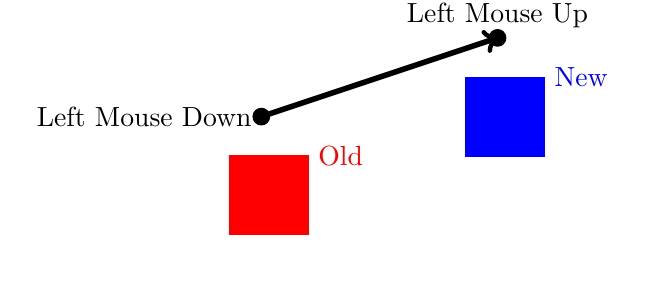
\begin{tikzpicture}
	\filldraw [color=red] (0, 1) rectangle (1, 2) node [pos=1,right] {Old};
	\filldraw [color=blue] (3, 2) rectangle (4, 3) node [pos=1,right] {New};
	\draw [color=black, line width=0.7mm, ->] (0.4, 2.5) -- (3.4, 3.5);
	\filldraw 
	(0.4, 2.5) circle (3pt) node[left] {Left Mouse Down} --
	(3.4, 3.5) circle (3pt) node[above] {Left Mouse Up};
\end{tikzpicture}

\subsubsection{Rotation}

For example, suppose we want to rotate polygon 4. 

\begin{enumerate}
\item Select ``Rotation $\to$ Rotate 4'' on menu bar OR press
	\lstinline{r} and then \lstinline{4} on keyboard. 
\item Drag the mouse from point $a$ to point $b$ on the screen. Suppose the
	centroid of polygon 4 is $c$, then the rotation angle will be the angle
	between vector $a - c$ and $b - c$. 
\end{enumerate}

See the figure below. 

\

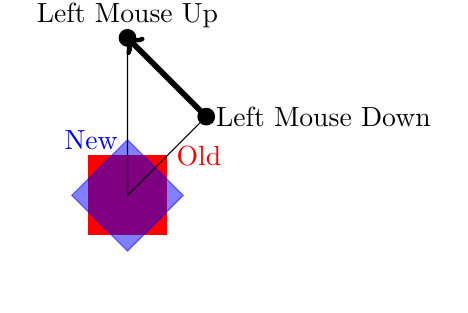
\begin{tikzpicture}
	\filldraw [color=red] (-.5, -.5) rectangle (.5, .5) node [pos=1,right] {Old};
	\filldraw [color=blue, opacity=0.5, rotate=45] (-.5, -.5) rectangle (.5, .5) node [pos=1, left, opacity=1] {New};
	\draw [color=black, line width=0.7mm, ->] (1, 1) -- (0, 2);
	\filldraw 
	(1, 1) circle (3pt) node[right] {Left Mouse Down} --
	(0, 2) circle (3pt) node[above] {Left Mouse Up};
	\draw (1, 1) -- (0, 0) -- (0, 2);
\end{tikzpicture}

\subsubsection{Scaling}

For example, suppose we want to scale polygon 2. 

\begin{enumerate}
\item Select ``Scaling $\to$ Scale 2'' on menu bar OR press
	\lstinline{r} and then \lstinline{2} on keyboard. 
\item Drag the mouse from point $a = (x_a, y_a)$ to point $b = (x_b, y_b)$ on
	the screen. Suppose the centroid of polygon 2 is $c = (x_c, y_c)$, then the
	x scaling factor will be $\displaystyle\frac{x_b - x_c}{x_a - x_c}$ and the
	y scaling factor will be $\displaystyle\frac{y_b - y_c}{y_a - y_c}$. 
\end{enumerate}

Note: try not to click on points that have close x or y values to the centroid,
 as this may make the polygon really big or small. 

See the figure below. 

\

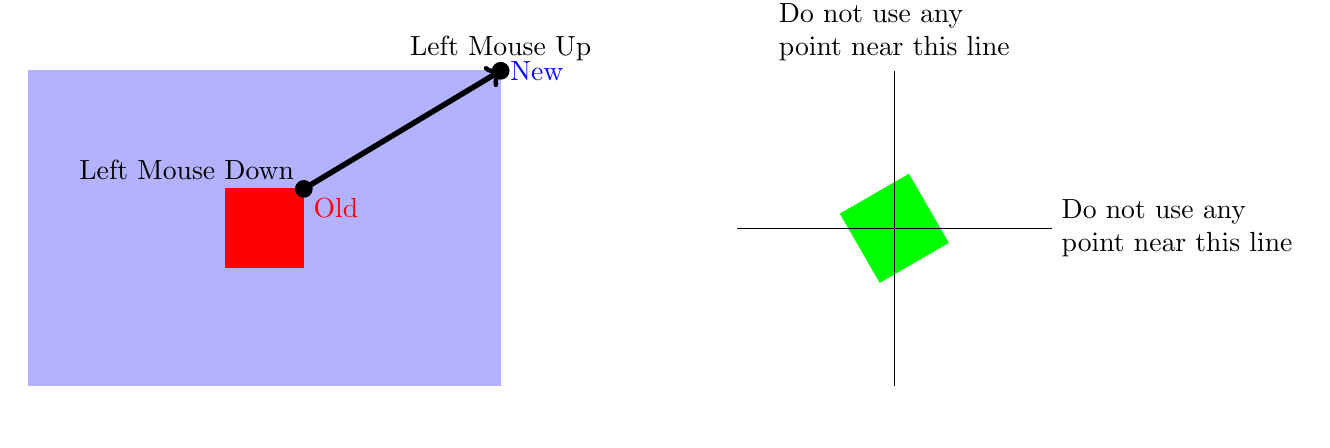
\begin{tikzpicture}
	\filldraw [color=blue!30!white] (-3, -2) rectangle (3, 2) node [pos=1,right, color=blue] {New};
	\filldraw [color=red] (-.5, -.5) rectangle (.5, .5) node [pos=1,below right] {Old};
	\draw [color=black, line width=0.7mm, ->] (0.5, 0.5) -- (3, 2);
	\filldraw 
	(0.5, 0.5) circle (3pt) node[above left] {Left Mouse Down} --
	(3, 2) circle (3pt) node[above] {Left Mouse Up};
	
	\def\x{8}
	\def\xx{\x*3^0.5/2}
	\def\yy{-\x*1/2}
	\filldraw [color=green, rotate=30] (\xx-.5, \yy-.5) rectangle (\xx+.5, \yy+.5);
	\draw (\x-2, 0) -- (\x+2, 0) node [pos=1, right, align=left] {
		Do not use any \\ point near this line}; 
	\draw (\x , -2) -- (\x , +2) node [pos=1, above, align=left] {
		Do not use any \\ point near this line}; 
	
\end{tikzpicture}

\subsection{Quitting}

Select ``Quit'' or press \lstinline{q} to quit. 

\section{Extra Features}

If you press \lstinline{K} (Shift + K) on keyboard, everything will rotate. This
 is just for fun. Press \lstinline{K} (Shift + K) again to stop this behavior. 

In my program, the \lstinline[language=c]{draw_pix()} function is passed into
 DDA and Bresenham through a function pointer of type
 \lstinline[language=c]{void (*)(int, int)}. This gives the user more
 flexibility when using my library, and it allows me to highlight the polygon
 that is selected to be transformed. 

To implement the interactive rotation, there is conversion between
 $\alpha$ and $\sin(\alpha)$ and $\cos(\alpha)$ implemented. See program output
 when a rotation is completed. Sample output:
 ``Rotate cos = 0.670286; sin = -0.742103; angle = -47.910835 deg''

\section{Keyboard Summary}

\newcommand{\keyboard}[1]{
	Hide / show polygon #1 \  OR \  Select polygon #1 for transformation
}

\begin{tabular}{ | l | l | }\hline
Key choices		& Function \\ \hline
b / d / B / D	& Bresenham / DDA \\ \hline
f / F			& Fill / Draw \\ \hline
c				& Enable clip (select region using mouse) \\ \hline
C				& Disable clip \\ \hline
t / T			& Translation (specify vector using mouse) \\ \hline
r / R			& Rotation (specify angle using mouse) \\ \hline
s / S			& Scaling (specify factor using mouse) \\ \hline
K				& Automatically rotate (extra) \\ \hline
q / Q			& Quit \\ \hline
0				& \keyboard{0} \\ \hline
1				& \keyboard{1} \\ \hline
2				& \keyboard{2} \\ \hline
3				& \keyboard{3} \\ \hline
4				& \keyboard{4} \\ \hline
5				& \keyboard{5} \\ \hline
6				& \keyboard{6} \\ \hline
7				& \keyboard{7} \\ \hline
8				& \keyboard{8} \\ \hline
9				& \keyboard{9} \\ \hline
\end{tabular}

\end{document}

